\subsection{Motivation}
The goal behind our app was to create a simple yet powerful tool for crypto currency users, both novice and more experienced. The majority of wallets provide a backup
mnemonics passphrase, also known as a seed, to the user when they first create their wallet. These mnemonic passphrase's are used to deterministically generate the public/private key
pairs that correspond to the users addresses. Since the mnemonic phrases are used to generate addresses deterministically, it's often the case that they correspond to multiple
cryptocurrencies. The hardware wallets trezor and ledger for example have a single seed that can correspond to multiple crypto currencies. The seed is a convenient way of being able
to recover funds or move funds to a different hardware wallet. If used correctly, they can also make losing funds extremely difficult- i.e. they are backed up. It can be easy to misplace the seed, and
they are unfortunately not immune to fire, natural disasters, home invasions. With the surge of interest in crypto there have consequently been an uptick in robberies as well as people
coming out announcing they lost X bitcoins on an old hard drive. Stegoshares provides a safe and convenient way of distributing ones seed for later use.


\begin{figure}[H]
\centering
\begin{minipage}{.5\textwidth}
  \centering
  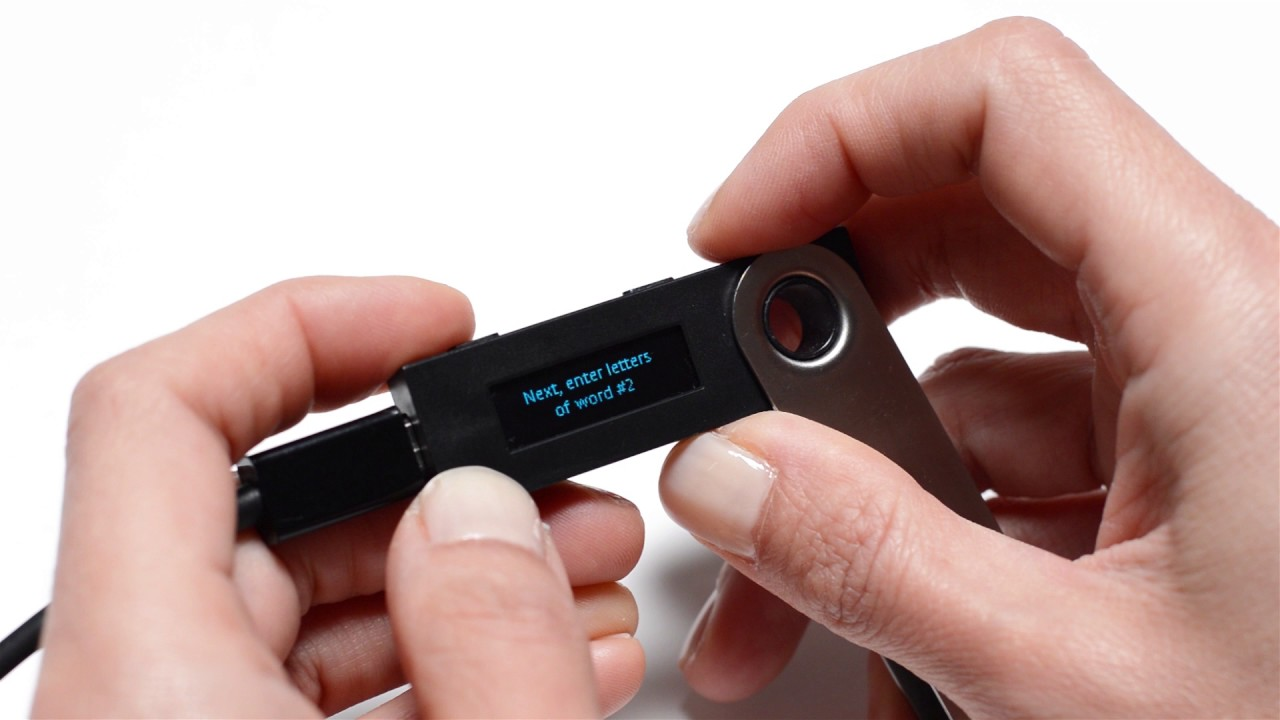
\includegraphics[scale = 0.15]{ledgerPhrase.jpg}
	\caption{Hiding Phase of Stegoshare}
	\label{fig: Hiding Phas}
\end{minipage}%
\begin{minipage}{.5\textwidth}
  \centering
  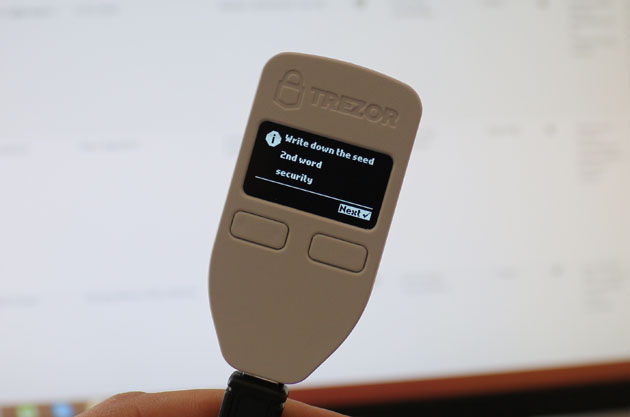
\includegraphics[scale = 0.25]{trezorPhrase.jpg}
	\caption{Recovery Phase of Stegoshare}
	\label{fig: Recovery Phas}
\end{minipage}
\end{figure}

\newpage
\subsection{Our Solution}
Stegoshare provides a trustless, and simple way to store crypto currency seeds in the form of multiple pictures. We believe that remembering pictures is inherently easier then remembering
a string of unconnected words. These pictures store shares using shamirs secret sharing algorithm that allow for the recovery of the original mnemonic seed. There is an option to additionally encrypt
the shares as well-adding an additional layer of security. The images are stored as .png to prevent loss of data that a format like jpeg causes due to compression. The user is then able to distribute these
images to locations of their choices such as cloud provides, usbs, etc. 

\begin{figure}[H]
\centering
\begin{minipage}{.5\textwidth}
  \centering
	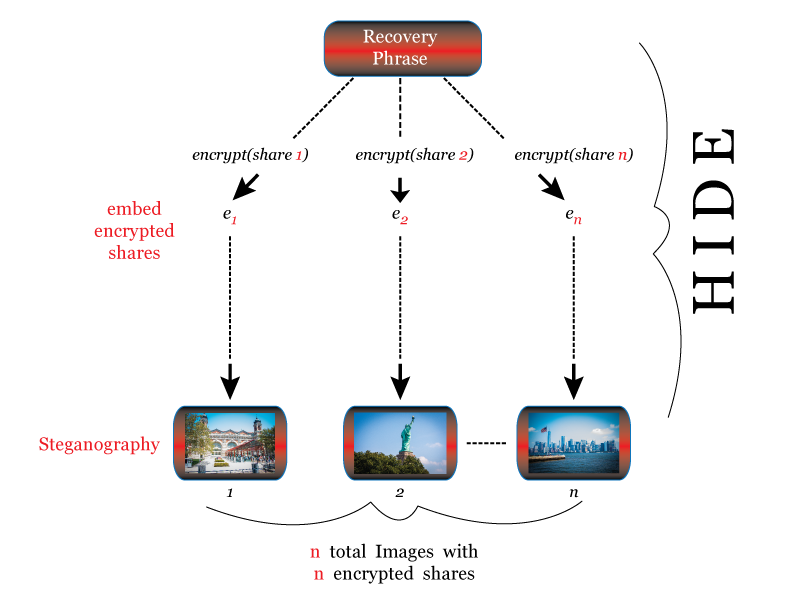
\includegraphics[scale = 0.29]{hide_slide-3.png}
	\caption{Hiding Phase of Stegoshare}
	\label{fig: Hiding Phas}
\end{minipage}%
\begin{minipage}{.5\textwidth}
  \centering
	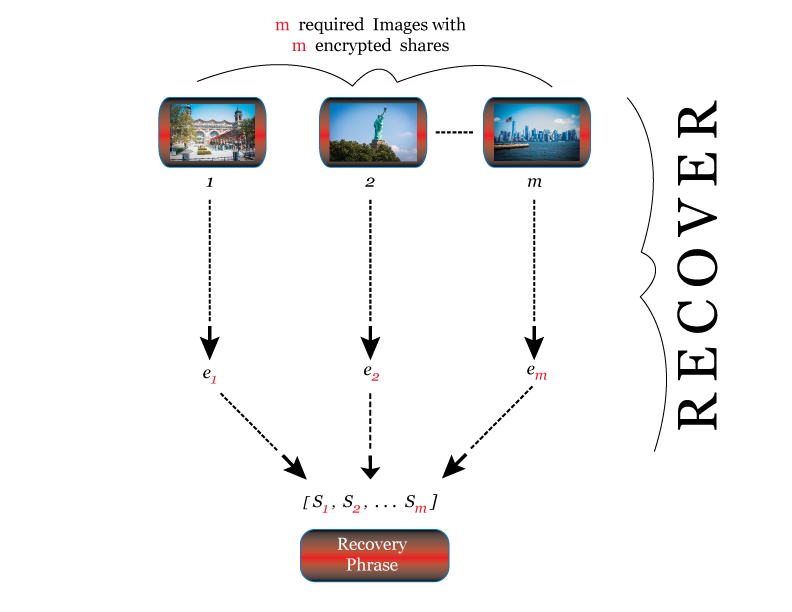
\includegraphics[scale = 0.29]{recover_slide-3.png}
	\caption{Recovery Phase of Stegoshare}
	\label{fig: Recovery Phas}
\end{minipage}
\end{figure}
